\documentclass[11pt,a4paper]{article}
\usepackage[margin=2.3cm]{geometry}
\usepackage{times}
\usepackage[T1]{fontenc}
\usepackage{microtype,booktabs,graphicx,amsmath,enumitem,float}
\usepackage[authoryear,round]{natbib}
\usepackage[colorlinks=true,linkcolor=blue,citecolor=blue,urlcolor=blue]{hyperref}
\usepackage{tikz}
\usetikzlibrary{arrows.meta,positioning,fit}
\newcommand{\MODELF}{0.805}
\newcommand{\VZERO}{0.800 $\pm$ 0.010}
\newcommand{\CENTRAL}{0.850 $\pm$ 0.007}
\newcommand{\TEMP}{1.22}
\newcommand{\ECEB}{0.050}
\newcommand{\ECEA}{0.029}
\newcommand{\NLLB}{0.409}
\newcommand{\NLLA}{0.388}
\newcommand{\RESULTSKEW}{%
Plain federated averaging stayed close to where it started. At the default $\alpha=0.5$ FedAvg reaches 0.800 on two seeds, the same as v0 (0.800 on three seeds), and well below centralised training on all data (0.850). The pairs per seed show why there is no gain to report: on seed 42 federation improved on v0 by 1.7 points (0.788 to 0.805), on seed 43 it lost 0.3 (0.798 to 0.795). With two seeds that is no detectable gain. With FedAvg, the 60\% of the training photos held by the farms added nothing that the 40\% central pool had not already given the model, under these settings (30 rounds, one local epoch, local learning rate $10^{-5}$ chosen in a short pilot of three values).

Label skew has a mild effect. From almost identical clients ($\alpha=100$) to strongly skewed ones ($\alpha=0.1$) the means fall from 0.794 to 0.779, but the $\alpha=100$ cell is not better than $\alpha=0.5$ and the two seeds differ from each other by as much as the cells do, so only the most skewed setting stands out, and only just. FedProx, which pulls each local model back towards the global one, does better. At $\alpha=0.5$ it reaches 0.811 on both seeds (0.812 and 0.810), above FedAvg on each seed (by 0.7 and 1.5 points) and above v0 on each seed (by 2.4 and 1.2 points). It is the only federated setting here that beats the central starting model on every seed it was run on. This rests on two seeds, so it is a consistent sign and not a firm ranking. At $\alpha=0.1$ FedProx was run on one seed only (0.801 against 0.797 for FedAvg on that seed), which cannot be separated from noise.}

\newcommand{\RESULTSCOPE}{%
Training and sending only the last blocks (430\,k parameters, 1.72 MB) gives 0.803 and the classifier head alone (20\,k parameters, 80 KB) gives 0.796, against 0.800 for the whole network (8.84 MB). The three differ by at most 0.007, about the seed-to-seed spread (0.003 to 0.005), so the cheapest scope gives up nothing measurable here. Over 30 rounds a client would upload about 265 MB for the full network and 2.4 MB for the head. For farms on slow rural connections this is the result that matters most: it makes the update small enough to send, at no cost in accuracy that these runs can detect.

The central stage is not optional. Starting from the ImageNet backbone with an empty head, the full network reaches only 0.287 after 30 rounds on both seeds (validation macro-F1 was still rising slowly, 0.30 at the last round). Federated learning with 10 clients, one local epoch and this learning rate does not rebuild what central pre-training provides in a few thousand images.}

\newcommand{\RESULTCLASS}{%
The tuber classes with enough photos are reliable (F1 at or above 0.93 for Blackspot Bruising, Brown Rot, Dry Rot, Healthy and Soft Rot). The weak spot is the leaf classes that look alike: Fungi, Pest and Phytophthora score 0.62 to 0.67, and the confusion matrix shows why. Pest is read as Fungi in 25 of 89 test photos, and Fungi as Phytophthora or Pest in 17 and 16 of 109. Two rare tuber classes, Blackleg and Common Scab, score 0.59 and 0.55 but have 7 test photos each, so those two scores can move by several points with one photo. This is why the service reports a tier and not just a label: 11 of the 16 held-out sample photos were ``very likely'' and correct, and the 4 wrong ones were all ``possible''.}

\newcommand{\CONCLUSION}{%
The deliverable is a working end-to-end system: a scripted pipeline from raw photos to a calibrated model, a containerised API that answers with a class, a confidence tier and a heat-map, drift monitoring on the inputs, tests, and instructions that let a reviewer check it in minutes (a mini-dataset smoke run, a 25-minute real federated run from the shipped starting model) or rerun the whole grid.

The experiments give three findings. First, centralised training on all the photos (0.850) is better than anything federated here: FedAvg gives about 0.80 and FedProx at $\alpha=0.5$ gives 0.811, so federation cost four to five points of macro-F1 and recovered at most one to two points of the five-point gap between the central starting model and centralised training. Second, label skew matters less than the choice of starting point; without the central stage the full network fails (0.287). Third, the cheapest update, the classifier head at 80 KB, is as good as the whole network at 8.84 MB, so communication cost does not have to be paid for accuracy.

What this does not show is how the system behaves on photos from real Kenyan farms, since the clients are simulated from two public datasets and the test set comes from the same sources. The drift monitor is the part of the system built for that gap.}

\setlength{\parskip}{0.45em}
\setlength{\parindent}{0pt}
\graphicspath{{../results/}}

\title{\textbf{Federated Deep Learning for Privacy-Preserving Potato Disease Detection:\\ a Pipeline and Model Service}\\[0.3em]\large DSA 8401 Applied Machine Learning, Capstone Report}
\author{Gracious Chepkemoi Ngetich\\MSc Data Science and Analytics, Strathmore University (iLabAfrica)}
\date{November 2026}

\begin{document}
\maketitle

\begin{abstract}
\noindent Late blight, bacterial wilt and tuber rots are hard for Kenyan smallholders to tell apart early, and the laboratory tests that confirm them destroy the sample. This project delivers an end-to-end system that classifies a photo of a potato leaf or tuber into 16 classes, trained with federated learning so that no farm has to hand over its photos. The system has a scripted pipeline (ingest and clean, central pre-training, federated training of the whole MobileNetV2, calibration), a FastAPI service in Docker that returns the class, a calibrated confidence tier and a Grad-CAM heat-map, and an Evidently AI drift monitor. On a held-out test set the shipped federated model (seed 42) reaches macro-F1 \MODELF. Averaged over seeds, FedAvg (about 0.80) matches the central starting model (\VZERO), FedProx at $\alpha=0.5$ is slightly above it (0.811 on two seeds), and all stay below centralised training on all data (\CENTRAL). The experiments show where federation helps and where it does not, and the report states the limits of what simulated clients on two public datasets can show.
\end{abstract}

\section{Problem and why it matters}
The system takes a photograph of a potato leaf or tuber and returns one of 16 classes: seven leaf classes (bacterial, fungal, nematode, pest, \emph{Phytophthora}, virus damage, healthy) and nine tuber classes (black scurf, blackleg, blackspot bruising, brown rot, common scab, dry rot, pink rot, soft rot, healthy). Potato is a main food and cash crop in Kenya, and the National Potato Strategy names late blight and bacterial wilt as major losses and the informal seed system as the route by which disease spreads \citep{potatos2021strategy}. The confirmatory tests destroy the sample and need equipment farmers lack, so a cheap first screen on a phone photo is useful, provided it says how sure it is.

Image models are usually trained on all photos pooled on one server. Cooperatives and county offices are unlikely to agree to that, so the project uses federated learning: each client trains on its own photos and sends only a model update to a server that averages them \citep{mcmahan2017communication}. Clients differ in disease mix, which breaks the assumption of identically distributed data behind federated averaging \citep{hsu2019measuring,li2020federated}. The central question is how much accuracy federation costs relative to central training, and which settings recover it.

\section{Data}
Two public datasets are used: potato leaf disease photographed in uncontrolled field conditions \citep{shabrina2023potato} and potato tuber disease \citep{islam2025potatocare}. Neither is a pre-cleaned benchmark, and the \texttt{ingest} stage documents what was wrong with them (Table~\ref{tab:clean}).

\begin{table}[H]\centering\small
\begin{tabular}{lrr}\toprule & Leaf & Tuber \\\midrule
Raw photos & 3,076 & 3,905 \\
Catch-all class removed (\emph{Miscellaneous}) & 0 & 74 \\
Byte-identical, conflicting labels & 12 & 26 \\
Byte-identical copies, same class & 49 & 0 \\
Near-identical (dHash $\le$ 4 of 64 bits), conflicting & 0 & 4 \\
Near-identical, same class & 36 & 7 \\\midrule
\textbf{Kept} & \textbf{2,979} & \textbf{3,794} \\
Class imbalance (largest : smallest) & 10.9 : 1 & 30.0 : 1 \\\bottomrule
\end{tabular}
\caption{What the cleaning stage removed. Every removed file and its reason is listed in \texttt{removed\_files.csv}.}\label{tab:clean}
\end{table}

The cleaning matters because duplicates that straddle the train and test split inflate scores, and because a copy filed under two diseases is a wrong label for one of them. Leaf photos are 1,500 px and tuber photos 224 px, so everything is resized to 128 px for training. Two further complications are introduced on purpose. First, class imbalance is kept and handled with capped inverse-frequency loss weights and macro-F1 as the headline metric. Second, because neither dataset is from Kenyan farms, the clients are simulated with a Dirichlet label-skew split whose parameter $\alpha$ is varied \citep{hsu2019measuring}: $\alpha=100$ is nearly identical clients, $\alpha=0.1$ gives each client a few dominant classes.

A stratified 70/15/15 split into train, validation and test is made once per seed and never used for tuning on the test part. Of the training images, 40\% form a central pool used to train the starting model v0; the other 60\% are divided among 10 simulated clients. The test set has 1,016 photos.

\section{Methods and why these}
\paragraph{Model.} A MobileNetV2 pretrained on ImageNet \citep{sandler2018mobilenetv2} with global average pooling, dropout and a 16-way softmax head, 2.28 M parameters. It is small enough for a phone and for repeated federated rounds on a laptop CPU.

\paragraph{Pipeline.} \texttt{ingest} cleans the data; \texttt{central} trains v0 on the 40\% pool (5 epochs of head training then 25 epochs of full fine-tuning with cosine decay, best validation macro-F1 kept) and, separately, the centralised reference on all training photos; \texttt{federate} runs the grid below; \texttt{bundle} calibrates and exports the shipped model; \texttt{report} produces every table and figure in this document from the run records.

\paragraph{Federated training.} Every trainable weight of the network is trained on the clients (BatchNorm layers keep their v0 statistics and are not exchanged) and averaged by the server weighted by client size (FedAvg). Each round every client does one local epoch with Adam and class-weighted loss, for 30 rounds. FedProx adds a proximal term with $\mu=0.1$ to keep local models near the global one \citep{li2020federated}. The local learning rate was chosen on validation macro-F1 in a pilot of 6 rounds over $10^{-5}, 3\times10^{-5}, 10^{-4}$; $10^{-5}$ won, and larger rates made the full network drop below v0 in the first rounds. Runs checkpoint every round and resume after interruption.

\paragraph{Grid.} (i) $\alpha\in\{100,1,0.5,0.1\}$ with FedAvg; (ii) FedProx at $\alpha\in\{0.5,0.1\}$; (iii) no central stage (ImageNet backbone, empty head) at $\alpha=0.5$; (iv) update scope: full network, last blocks only (about 20\% of parameters) or the classifier head only, at $\alpha=0.5$. The seed fixes the split, the client partition and the initialisation. Seed 42 was run for every cell and seed 43 for every cell except FedProx at $\alpha=0.1$; the number of seeds is given in every table. Standard deviations are over seeds.

\paragraph{Calibration.} A softmax score is not a probability \citep{guo2017calibration}. One temperature is fitted on the validation split by minimising log-loss; the test set then checks the expected calibration error (ECE) and the accuracy within three confidence tiers shown to the user.

\paragraph{Explanation.} Grad-CAM \citep{selvaraju2017gradcam} highlights the region that drove the prediction. For global average pooling followed by a linear head, the gradient of class $c$'s logit with respect to each feature-map cell is $W_{\cdot c}/(hw)$, so the heat-map is the feature map weighted by the class's head weights and needs no backward pass. A unit test compares it with autograd Grad-CAM.

\paragraph{Techniques left out, and why.} \emph{Vision Transformers and larger CNNs}: too heavy for phones on slow rural links, and no evidence they would help on 7,000 images. \emph{LLM, RAG or agent components}: nothing in an image classification task for them to do. \emph{SHAP}: Grad-CAM answers ``where in the photo'' directly and cheaply; pixel-level SHAP would cost hundreds of forward passes per request. \emph{Gradient boosting or classical models on hand features}: leaf and tuber disease differ in texture and shape that pretrained convolutional features capture far better. \emph{Sample-level DP-SGD or secure aggregation}: they protect against a different threat from the one this system addresses (the server seeing raw photos), and with 10 clients the privacy budget would be too weak to claim anything; the system therefore makes no formal privacy guarantee beyond ``photos never leave the client''. \emph{Other FL algorithms (SCAFFOLD, FedAdam)}: FedAvg and FedProx cover the standard baseline and the standard heterogeneity fix; adding more would not change the deployment.

\section{System}
\begin{figure}[H]\centering
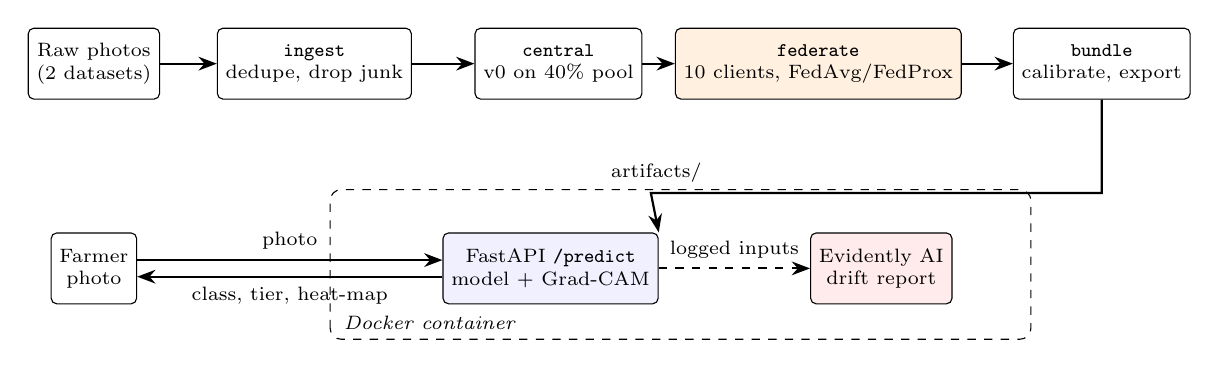
\begin{tikzpicture}[font=\scriptsize, box/.style={draw, rounded corners=2pt, align=center, inner sep=3pt, fill=white, minimum height=0.9cm}, arr/.style={-{Stealth}, thick}]
\node[box] (raw) at (0.2,0) {Raw photos\\(2 datasets)};
\node[box] (cl) at (3.0,0) {\texttt{ingest}\\dedupe, drop junk};
\node[box] (v0) at (6.1,0) {\texttt{central}\\v0 on 40\% pool};
\node[box, fill=orange!12] (fl) at (9.4,0) {\texttt{federate}\\10 clients, FedAvg/FedProx};
\node[box] (bd) at (13.0,0) {\texttt{bundle}\\calibrate, export};
\draw[arr] (raw)--(cl); \draw[arr] (cl)--(v0); \draw[arr] (v0)--(fl); \draw[arr] (fl)--(bd);
\node[box] (ph) at (0.2,-2.6) {Farmer\\photo};
\node[box, fill=blue!6] (api) at (6.0,-2.6) {FastAPI \texttt{/predict}\\model + Grad-CAM};
\node[box, fill=red!8] (mon) at (10.2,-2.6) {Evidently AI\\drift report};
\draw[arr] (bd.south) |- ([yshift=0.5cm]api.north east) -- node[above, pos=0.3]{artifacts/} ++(-0.1,0) -- (api.north east);
\draw[arr] ([yshift=3pt]ph.east)--node[above]{photo}([yshift=3pt]api.west);
\draw[arr] ([yshift=-3pt]api.west)--node[below]{class, tier, heat-map}([yshift=-3pt]ph.east);
\draw[arr, dashed] (api)--node[above]{logged inputs}(mon);
\draw[dashed, rounded corners] (3.2,-3.5) rectangle (12.1,-1.6);
\node[font=\scriptsize\itshape, anchor=south west] at (3.25,-3.5) {Docker container};
\end{tikzpicture}
\caption{Architecture. The top row is the scripted pipeline; the bottom row is the container that serves the artifacts.}
\end{figure}

\paragraph{Service.} \texttt{POST /predict} accepts a JPEG or PNG, fixes EXIF rotation, resizes to 128 px and returns the top three classes with calibrated probabilities, a tier (\emph{very likely} from 0.90, \emph{possible} from 0.50, otherwise \emph{unsure}), a sentence of advice for the tier and, on request, the heat-map blended over the photo as a PNG. Non-images and photos under 64 px get a 422 and files over 10 MB a 413. \texttt{GET /model} reports the version, temperature and test metrics; \texttt{GET /healthz} is the liveness check used by the container. The container is built from \texttt{python:3.12-slim} with the model bundle copied in (9.7 MB), so a reviewer needs only \texttt{docker compose up}.

\begin{figure}[H]\centering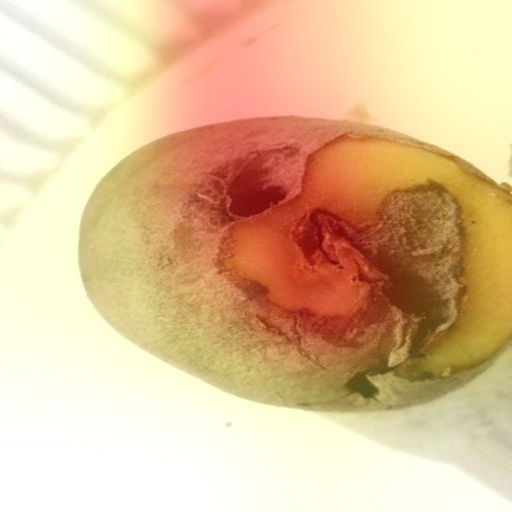
\includegraphics[width=0.36\linewidth]{fig_cam.png}\caption{Heat-map returned by the service for a held-out dry-rot tuber (predicted Dry Rot, 99\% confidence): the highlight sits on the lesion.}\end{figure}

\paragraph{Monitoring.} The service never sees the true label, so accuracy cannot be tracked in production, but it can see the photo. Each request logs brightness, contrast, sharpness (variance of the Laplacian), saturation, green share and image size, plus the model's confidence. \texttt{GET /drift} compares the latest 500 requests with the same statistics of the training photos using Evidently's data-drift report. Each of the seven columns gets a two-sample Kolmogorov--Smirnov test, and a column counts as drifted when its $p$-value is below $0.05/7$ (a Bonferroni correction). The service reports drift when any column drifts, because a darker, blurrier or larger photo moves some columns and leaves others, such as colour ratios, untouched. \texttt{/drift/report} returns the full HTML report. On 60 to 70 photos sent to the running container, ordinary photos from the dataset gave no drift, very dark photos flagged brightness, contrast and sharpness, 3000-pixel photos flagged width and height, and blurred photos flagged sharpness. Windows drawn from the reference itself raised a false alarm in about 3\% of 240 trials.

\paragraph{Tests.} Twenty-one pytest cases cover the Dirichlet partition (disjoint cover, reproducibility, more skew at smaller $\alpha$), update compression and clipping, near-duplicate grouping, temperature recovery on synthetic over-confident logits, the API (valid input, heat-map, bad input, model card), drift detection (a dark window, a window where only sharpness shifts, and a clean window), the quality gate, and the Grad-CAM identity.

\section{Results}
All numbers are macro-F1 on the 1,016-photo test set; $\pm$ is the standard deviation over seeds; (n=\ldots) gives the number of seeds behind each cell. Results are those of the code in this repository (\texttt{results/fl\_full/core.jsonl}).

\subsection{Label skew and algorithm}
\begin{table}[H]\centering\small
\begin{tabular}{rrcc}
\toprule
$\alpha$ & label skew (JS) & FedAvg macro-F1 & FedProx macro-F1 \\
\midrule
100 & 0.00 & 0.794 $\pm$ 0.014 (n=2) & -- \\
1 & 0.11 & 0.808 $\pm$ 0.004 (n=2) & -- \\
0.5 & 0.13 & 0.800 $\pm$ 0.005 (n=2) & 0.811 $\pm$ 0.001 (n=2) \\
0.1 & 0.32 & 0.779 $\pm$ 0.018 (n=2) & 0.801 (n=1) \\
\midrule
\multicolumn{2}{l}{v0 (central pool only)} & \multicolumn{2}{c}{0.800 $\pm$ 0.010 (n=3)} \\
\multicolumn{2}{l}{Centralised, all data} & \multicolumn{2}{c}{0.850 $\pm$ 0.007 (n=3)} \\
\bottomrule
\end{tabular}
\caption{Federated full-network training: test macro-F1 by label skew and algorithm. $\alpha$ small means more skew; JS is the mean Jensen--Shannon divergence of client label mixes from the global mix.}\label{tab:skew}
\end{table}
\begin{figure}[H]\centering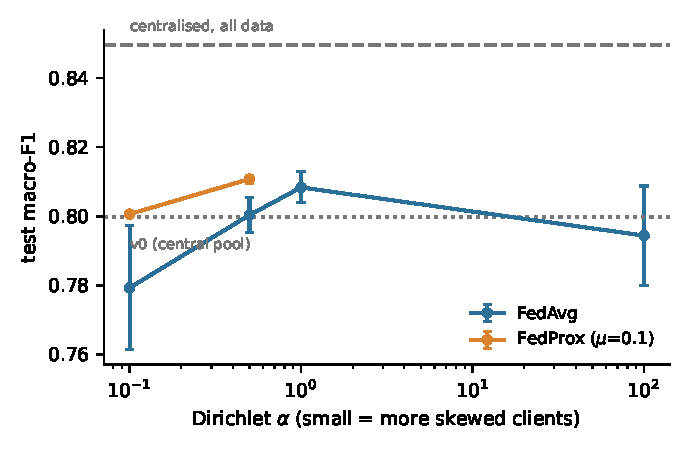
\includegraphics[width=0.62\linewidth]{fig_alpha.pdf}\caption{Test macro-F1 against Dirichlet $\alpha$. Dotted: v0. Dashed: centralised on all data.}\end{figure}

\RESULTSKEW

\subsection{Initialisation and update scope}
\begin{table}[H]\centering\small
\begin{tabular}{lrrc}
\toprule
Setting ($\alpha=0.5$) & parameters sent & MB per client per round & macro-F1 \\
\midrule
Full network from v0 (default) & 2,210,256 & 8.84 & 0.800 $\pm$ 0.005 (n=2) \\
Last blocks from v0 & 430,096 & 1.72 & 0.803 $\pm$ 0.003 (n=2) \\
Classifier head only from v0 & 20,496 & 0.08 & 0.796 $\pm$ 0.003 (n=2) \\
Full network, no central stage (empty head) & 2,210,256 & 8.84 & 0.287 $\pm$ 0.000 (n=2) \\
\bottomrule
\end{tabular}
\caption{What is trained and sent, at $\alpha=0.5$. ``Parameters sent'' is the update size per client per round.}\label{tab:scope}
\end{table}
\begin{figure}[H]\centering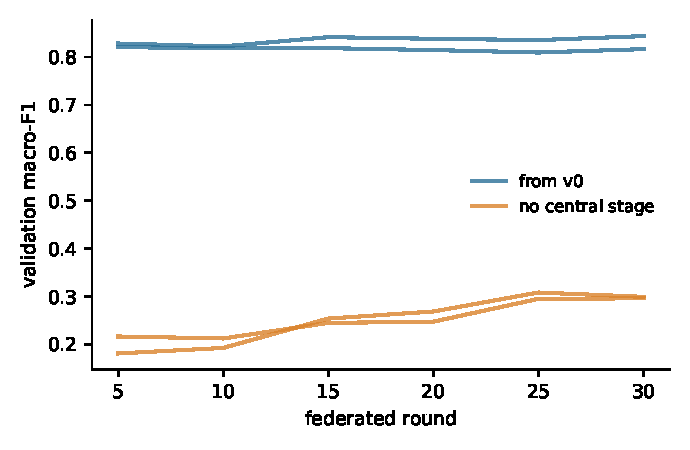
\includegraphics[width=0.48\linewidth]{fig_curves.pdf}\hfill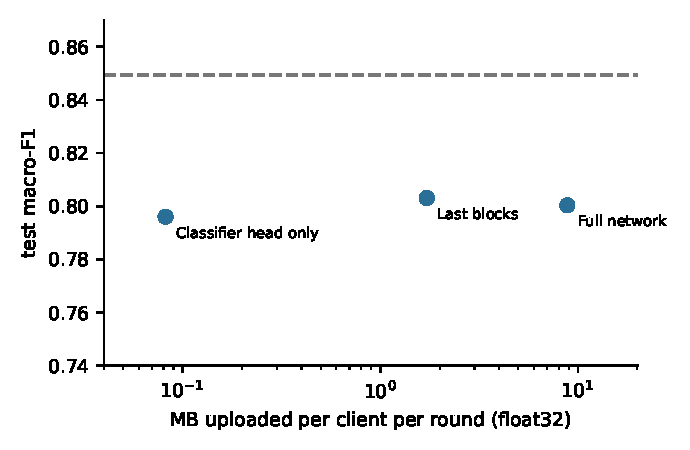
\includegraphics[width=0.48\linewidth]{fig_scope.pdf}\caption{Left: validation macro-F1 per round, from v0 (blue) and with no central stage (orange). Right: accuracy against upload size.}\end{figure}

\RESULTSCOPE

\subsection{The shipped model: per-class accuracy and calibration}
The shipped model is the FedAvg full-network model at $\alpha=0.5$, seed 42. Temperature scaling gives $T=\TEMP$ and lowers the expected calibration error from \ECEB{} to \ECEA{} and the test log-loss from \NLLB{} to \NLLA{}. The tiers behave as intended (Table~\ref{tab:tiers}): the farmer can rely on a ``very likely'' answer far more than on an ``unsure'' one.

\begin{table}[H]\centering\small
\begin{tabular}{lrr}\toprule Tier & share of test photos & accuracy in tier \\\midrule
very likely & 66.6\% & 97.6\% \\
possible & 27.9\% & 67.8\% \\
unsure & 5.5\% & 33.9\% \\
\bottomrule\end{tabular}
\caption{Calibrated confidence tiers on the test set.}\label{tab:tiers}
\end{table}

\begin{table}[H]\centering\small
\begin{tabular}{lrrrr}
\toprule
Class & precision & recall & F1 & test photos \\
\midrule
Leaf: Bacteria & 0.89 & 0.95 & 0.92 & 84 \\
Leaf: Fungi & 0.65 & 0.63 & 0.64 & 109 \\
Leaf: Healthy & 0.77 & 0.90 & 0.83 & 30 \\
Leaf: Nematode & 0.64 & 0.90 & 0.75 & 10 \\
Leaf: Pest & 0.69 & 0.56 & 0.62 & 89 \\
Leaf: Phytopthora & 0.62 & 0.74 & 0.67 & 46 \\
Leaf: Virus & 0.83 & 0.77 & 0.80 & 78 \\
Tuber: Black Scurf & 0.78 & 1.00 & 0.88 & 7 \\
Tuber: Blackleg & 0.50 & 0.71 & 0.59 & 7 \\
Tuber: Blackspot Bruising & 0.97 & 0.97 & 0.97 & 116 \\
Tuber: Brown Rot & 1.00 & 1.00 & 1.00 & 16 \\
Tuber: Common Scab & 0.75 & 0.43 & 0.55 & 7 \\
Tuber: Dry Rot & 0.97 & 0.96 & 0.97 & 203 \\
Tuber: Healthy Potatoes & 0.97 & 0.97 & 0.97 & 122 \\
Tuber: Pink Rot & 0.86 & 0.75 & 0.80 & 8 \\
Tuber: Soft Rot & 0.93 & 0.94 & 0.94 & 84 \\
\bottomrule
\end{tabular}
\caption{Per-class results of the shipped model on the test set.}\label{tab:perclass}
\end{table}

\RESULTCLASS

\section{Limitations}
\begin{itemize}[noitemsep]
\item The clients are simulated from two public datasets that are not Kenyan. The skew parameter varies the disease mix per client but not camera, lighting, season or geography, so the results bound the effect of label skew only.
\item The test photos come from the same two datasets as the training photos. Accuracy on photos taken in a farmer's field will be lower, and the drift monitor is there to notice when inputs move away from the training distribution; it cannot say whether accuracy fell.
\item Leaf photos are 1,500 px and tuber photos 224 px, so a model can partly tell the organ from image statistics. This does no harm for classification (leaf and tuber classes never compete) but it means the 16-class score is easier than a single-organ score would be.
\item Several classes have very few test photos (7 each for Blackleg, Black Scurf and Common Scab), so their per-class F1 is noisy.
\item Two seeds are enough to show that differences below about one point of macro-F1 cannot be told apart, not to rank closely spaced settings.
\item Federated learning here protects photos from being collected centrally. It gives no formal privacy guarantee on the updates, and the report makes no such claim.
\item The service is a screening aid. It is not a diagnosis and says so in its advice text.
\end{itemize}

\section{Conclusion}
\CONCLUSION

\paragraph{Reproducibility.} Everything is in one repository: \texttt{README.md} gives the commands for each stage and for \texttt{docker compose up}, \texttt{AI\_USE.md} discloses the AI assistance, and \texttt{tests/} holds the test suite.

\bibliographystyle{apalike}
\bibliography{references}
\end{document}
